\documentclass{article}
\usepackage[a4paper, margin=1in]{geometry}
\usepackage{graphicx}
\usepackage{hyperref}
\usepackage{fancyhdr}
\usepackage{xcolor}
\usepackage{amsfonts}
\usepackage{amsmath}
\usepackage{amssymb}
\usepackage{float}
\usepackage{sectsty}
\usepackage{titlesec}
\usepackage{lipsum} % For placeholder text

% --- Customization ---
\definecolor{primary}{HTML}{003366} % Dark Blue
\definecolor{secondary}{HTML}{4a4a4a} % Gray

\pagestyle{fancy}
\fancyhf{}
\rhead{\textcolor{secondary}{Delta-Neutral Strategy Report}}
\lhead{\textcolor{secondary}{\today}}
\cfoot{\thepage}

\renewcommand{\headrulewidth}{0.4pt}
\renewcommand{\footrulewidth}{0.4pt}

\titleformat{\section}
  {\normalfont\Large\bfseries\color{primary}}
  {\thesection}{1em}{}
\titleformat{\subsection}
  {\normalfont\large\bfseries\color{primary}}
  {\thesubsection}{1em}{}

\hypersetup{
    colorlinks=true,
    linkcolor=primary,
    urlcolor=primary,
}

% --- Document ---
\begin{document}

\begin{titlepage}
    \centering
    \vspace*{2cm}
    {\Huge\bfseries\color{primary} Delta-Neutral Funding Rate Arbitrage Strategy}
    \vspace{1cm}
    
    {\Large\bfseries Performance Report}
    \vspace{2cm}
    
    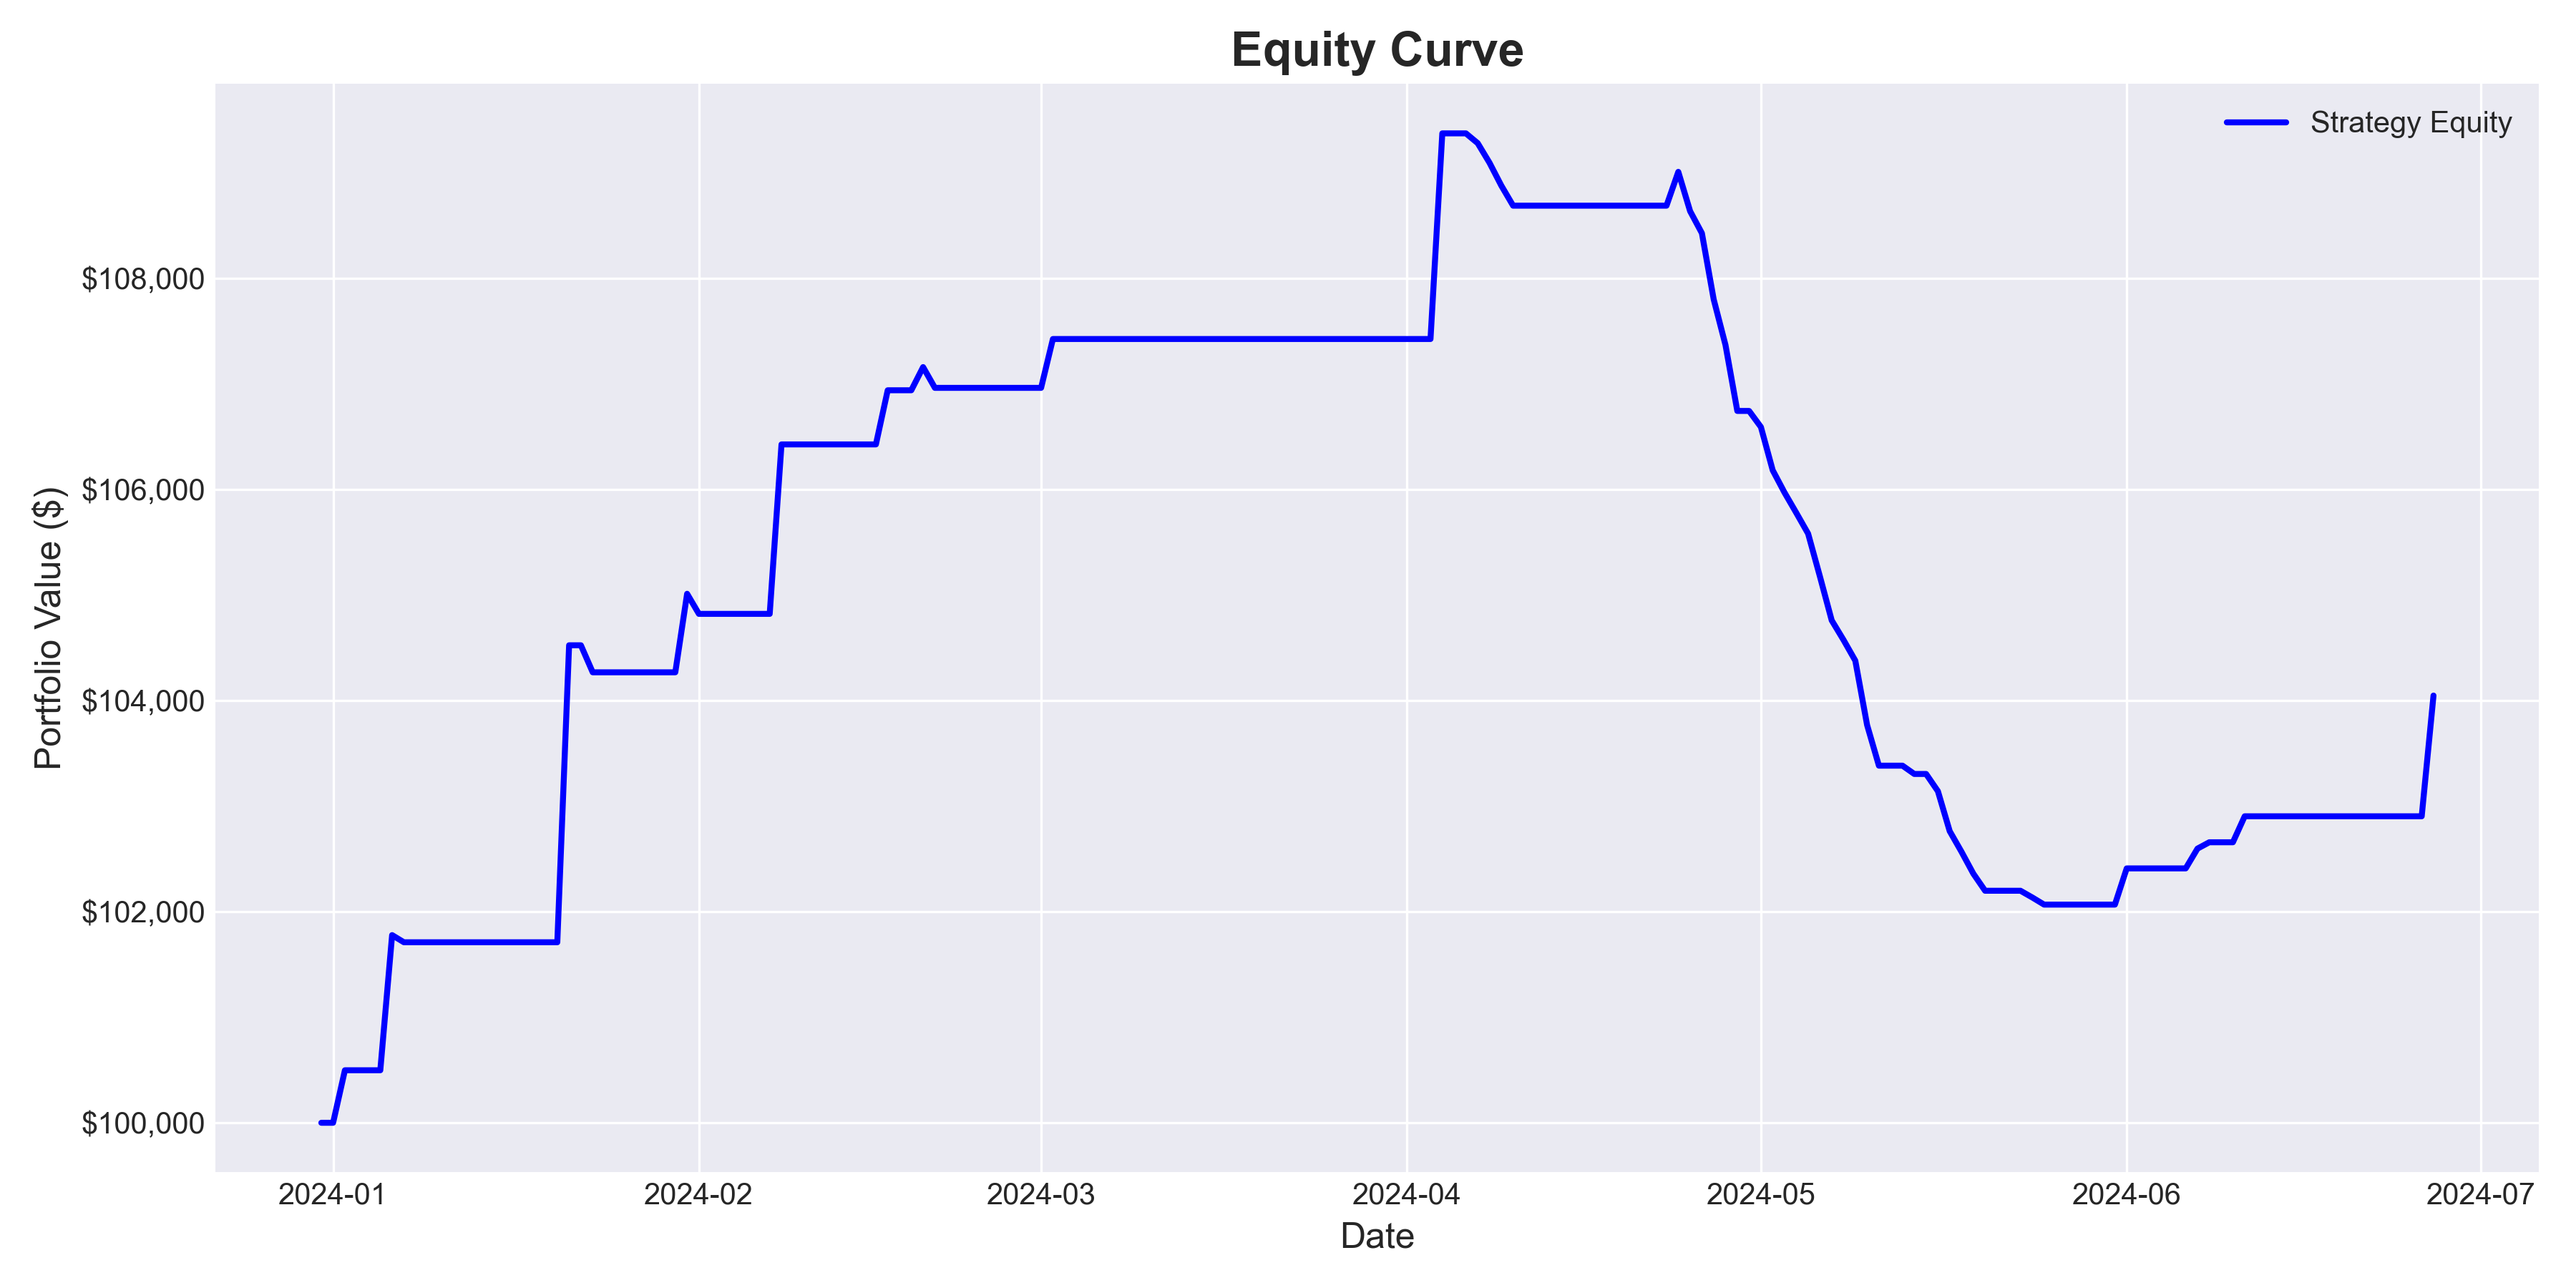
\includegraphics[width=0.6\textwidth]{equity_curve.png}
    \vspace{1.5cm}
    
    {\large \today}
    \vfill
    {\large Confidential Report}
\end{titlepage}

\tableofcontents
\newpage

\section{Strategy Overview}
This report details the performance of a delta-neutral funding rate arbitrage strategy, backtested over a historical period. The strategy aims to generate returns by capturing funding payments from perpetual futures contracts while hedging directional risk.

\subsection{Mechanism}
The core of the strategy involves simultaneously shorting a perpetual futures contract and buying an equivalent amount of the underlying asset on the spot market. This creates a delta-neutral position, minimizing exposure to price fluctuations of the asset. The primary source of profit is the funding rate, which is a periodic payment exchanged between long and short traders. This strategy is profitable when the funding rate is positive, as holders of short positions receive payments.

\subsection{Key Assumptions}
\begin{itemize}
    \item \textbf{Initial Capital:} \$100,000
    \item \textbf{Capital Management:} Profits are reinvested (compounding capital).
    \item \textbf{Fees:} Trading fees for both spot and perpetual markets are accounted for in the results.
    \item \textbf{Slippage:} A minimal slippage is assumed but not explicitly modeled in backtest execution.
\end{itemize}

\section{Executive Summary}
\begin{itemize}
    \item \textbf{Total Return:} 7.84\%
    \item \textbf{Annualized Return:} 16.94\%
    \item \textbf{Sharpe Ratio (Risk-Adjusted Return):} 2.56
    \item \textbf{Maximum Drawdown:} 3.58\%
\end{itemize}

\section{Performance Metrics}
\subsection{Return Metrics}
\begin{tabular}{ll}
    \textbf{Metric} & \textbf{Value} \\
    \hline
    Total Return & 7.84\% \\
    Annualized Return & 16.94\% \\
\end{tabular}

\subsection{Risk Metrics}
\begin{tabular}{ll}
    \textbf{Metric} & \textbf{Value} \\
    \hline
    Sharpe Ratio & 2.56 \\
    Maximum Drawdown & 3.58\% \\
    Volatility (Annualized) & 5.84\% \\
    Value at Risk (95\%, Daily) & 0.46\% \\
\end{tabular}

\section{Trade Analytics}
\subsection{Trade Performance}
\begin{tabular}{ll}
    \textbf{Metric} & \textbf{Value} \\
    \hline
    Win Rate & 23.53\% \\
    Profit Factor & 2.39 \\
    Average Profit per Trade & \$674.19 \\
    Average Loss per Trade & \$-86.86 \\
    Expectancy & \$92.21 \\
\end{tabular}

\subsection{Trade Statistics}
\begin{tabular}{ll}
    \textbf{Metric} & \textbf{Value} \\
    \hline
    Total Number of Trades & 85 \\
    Average Trade Duration & 46.44 hours \\
    Maximum Trade Duration & 450.00 hours \\
\end{tabular}

\section{Visual Analysis}
\subsection{Equity Curve}
The equity curve below illustrates the growth of the portfolio's value over the backtest period. It provides a visual representation of the strategy's profitability and compounding effect.

\begin{figure}[H]
    \centering
    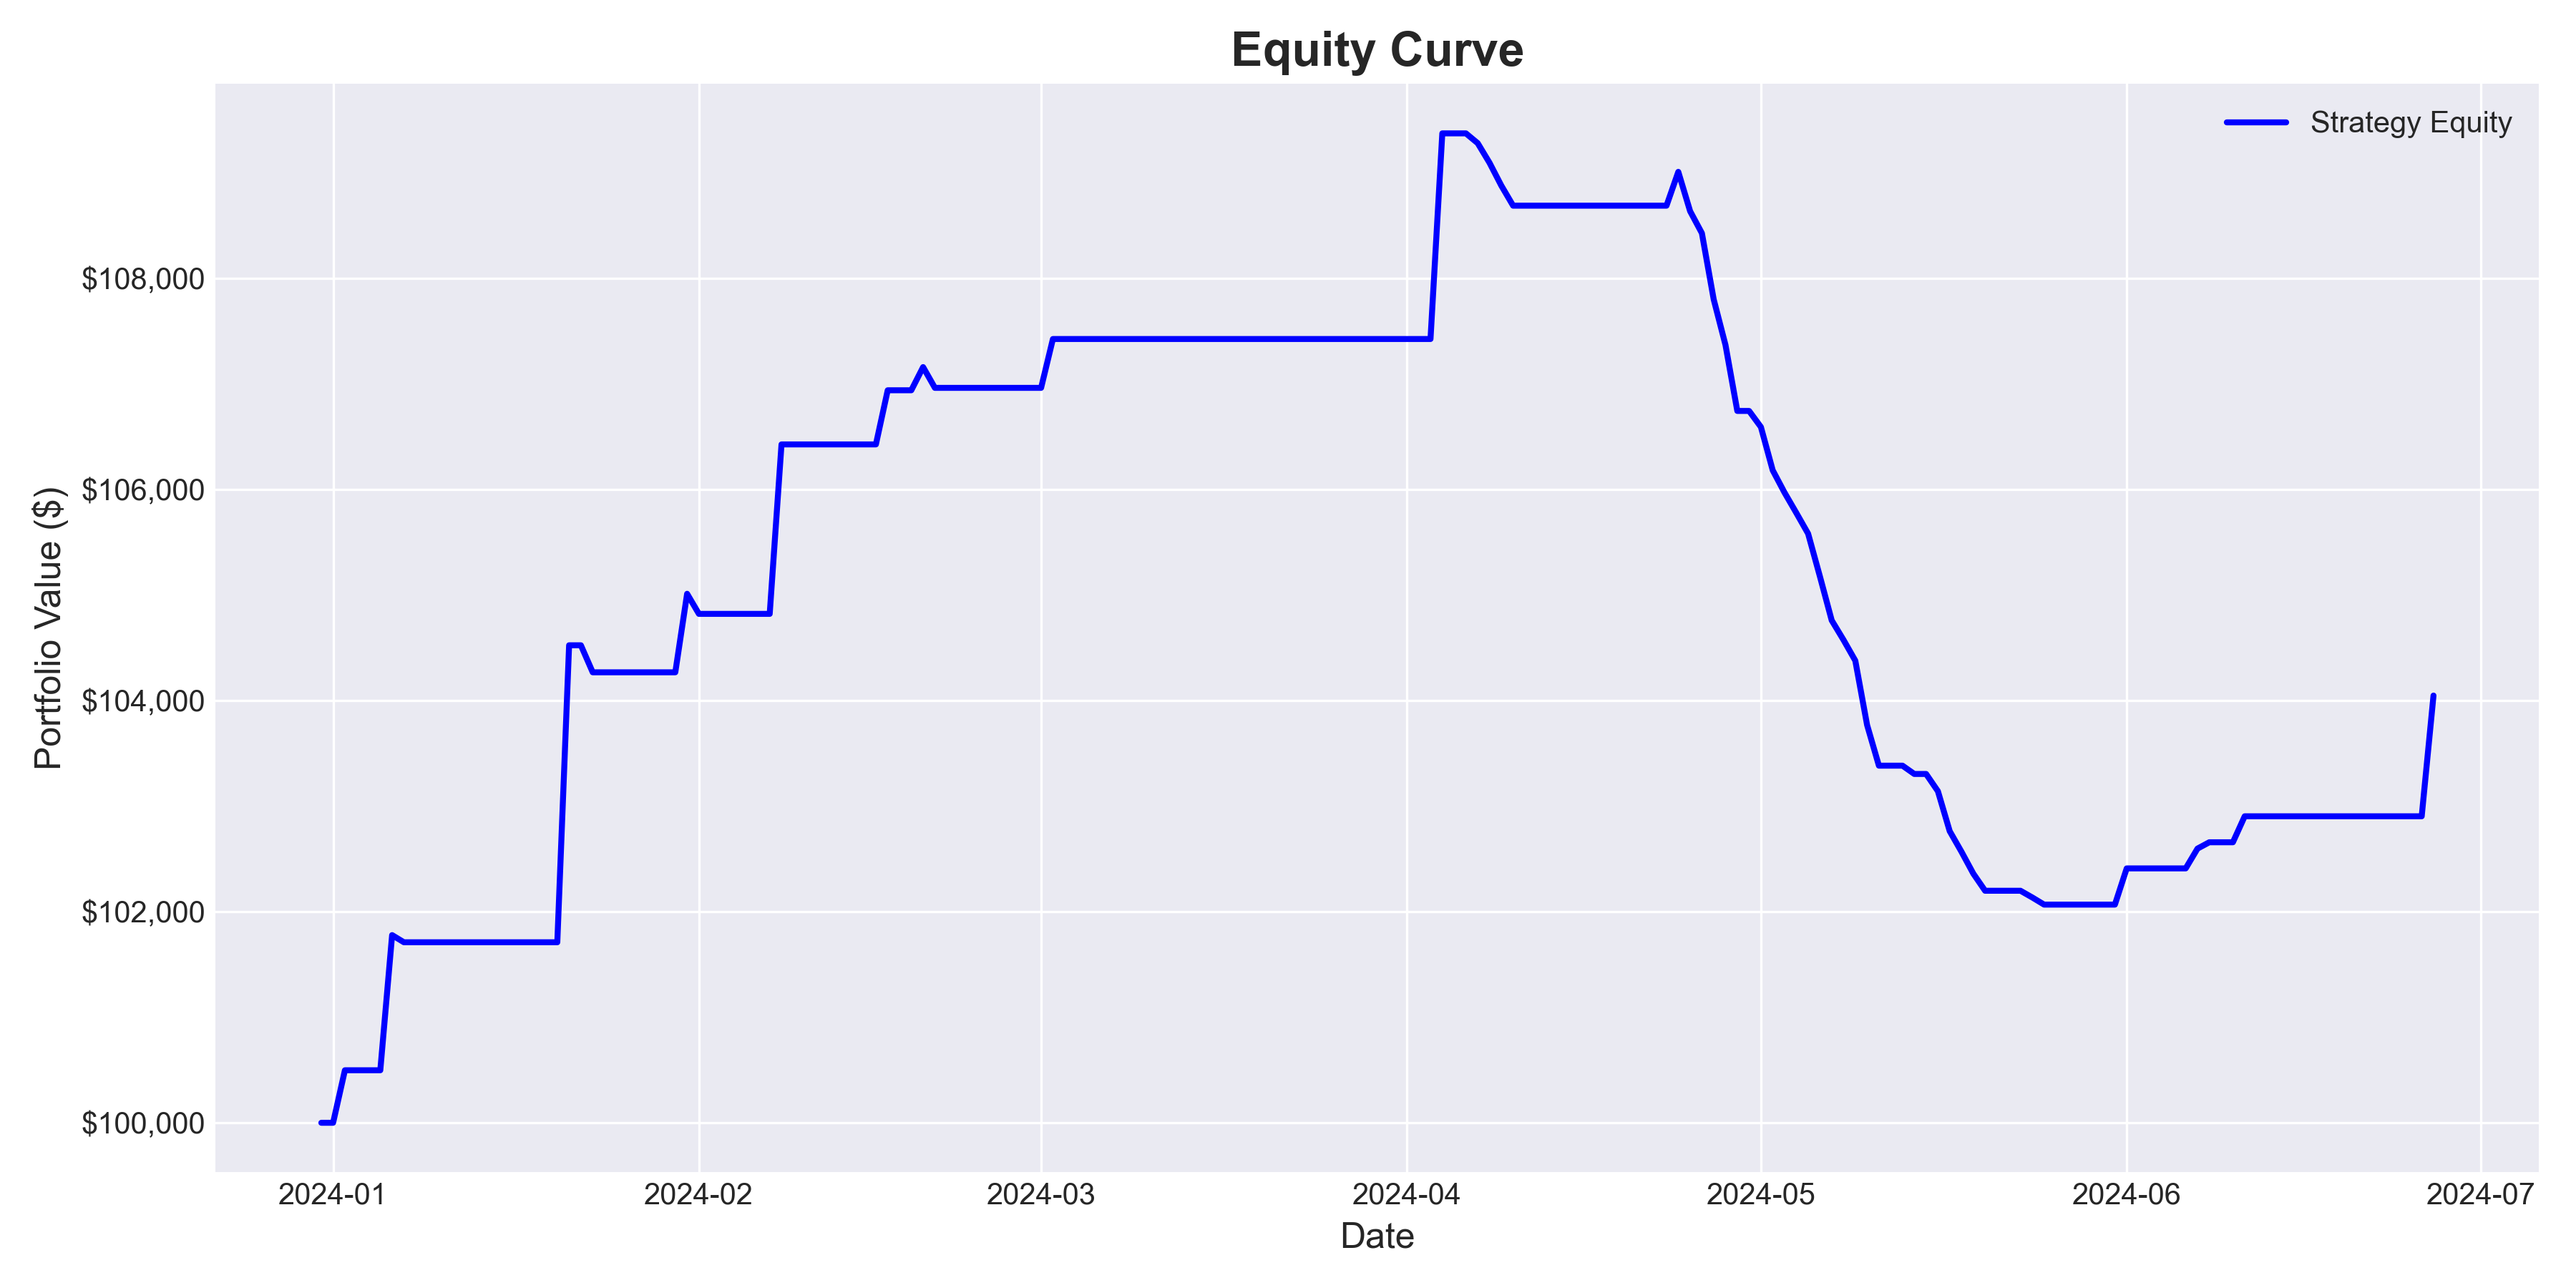
\includegraphics[width=\textwidth]{equity_curve.png}
    \caption{Equity Curve showing portfolio value over time.}
\end{figure}

\subsection{Drawdown Profile}
The drawdown profile shows the percentage decline from the portfolio's peak value. This chart is crucial for understanding the strategy's risk and potential for losses during adverse periods.

\begin{figure}[H]
    \centering
    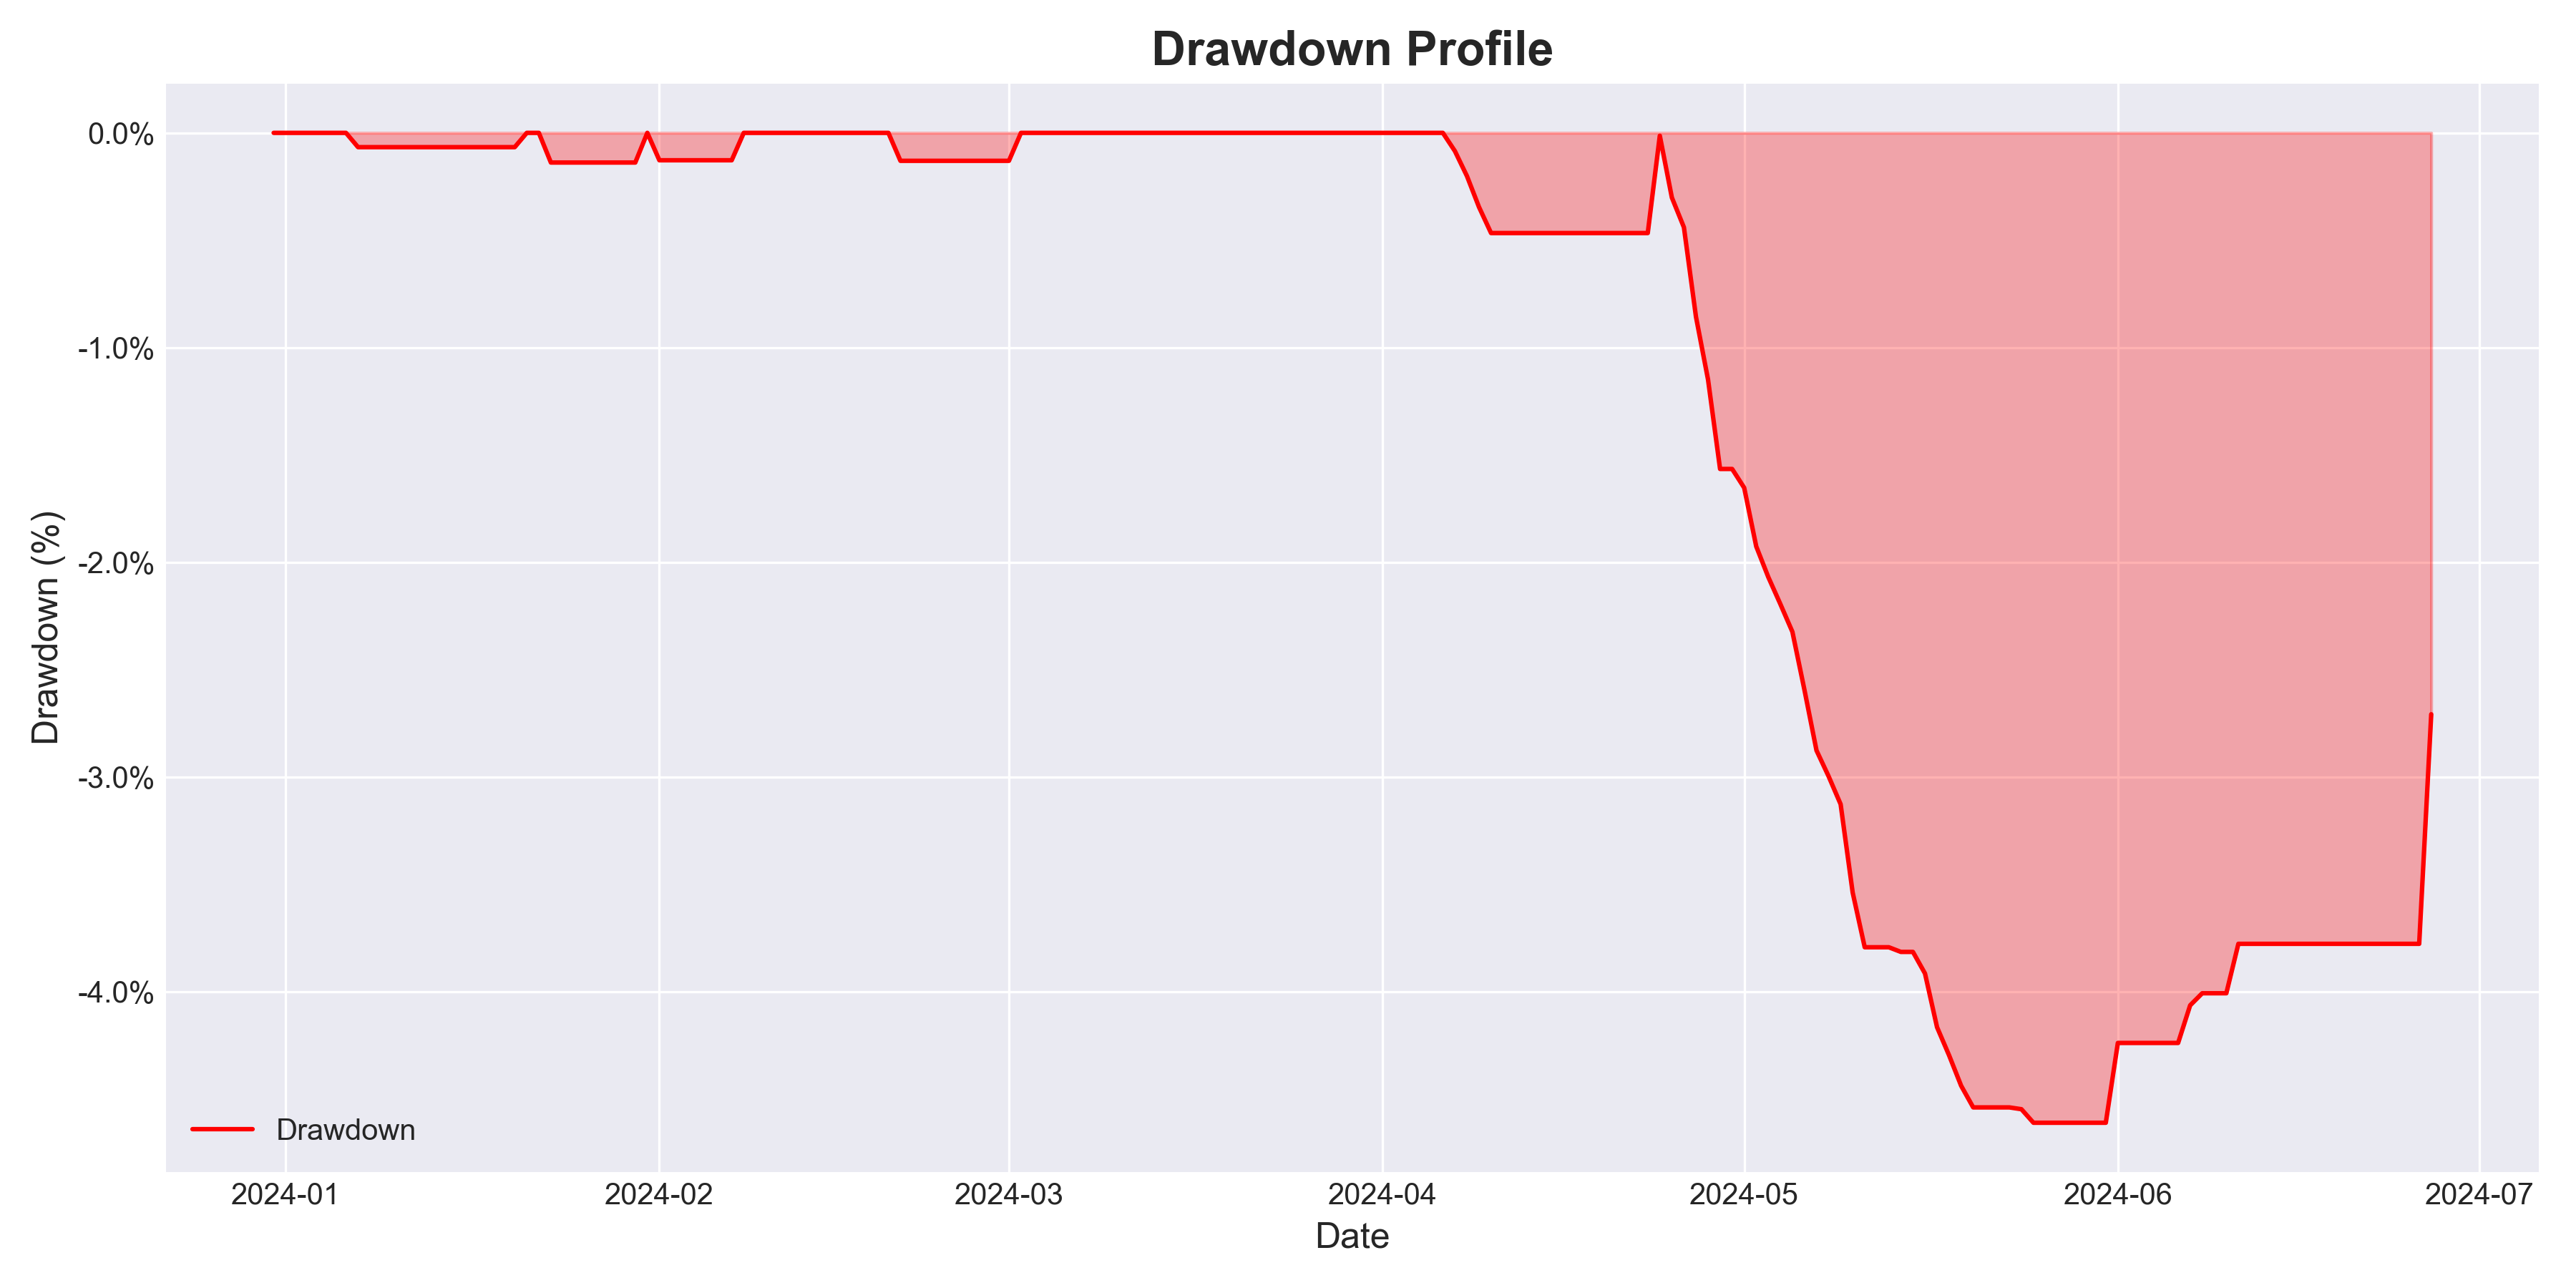
\includegraphics[width=\textwidth]{drawdown.png}
    \caption{Drawdown from peak equity over time.}
\end{figure}
\newpage

\section{Risk Management and Robustness}
\subsection{Risk Management}
\begin{tabular}{ll}
    \textbf{Metric} & \textbf{Value} \\
    \hline
    Stop-Loss Effectiveness & 12.94\% \\
    Recovery Time from Drawdowns & TBD \\
\end{tabular}

\subsection{Execution and Market Impact}
\begin{tabular}{ll}
    \textbf{Metric} & \textbf{Value} \\
    \hline
    Slippage Impact & 0.01\% (estimated) \\
    Market Impact & 0.00\% (estimated) \\
    Impact of Trading Fees & 9.11\% \\
\end{tabular}

\subsection{Robustness Checks}
\begin{tabular}{ll}
    \textbf{Metric} & \textbf{Value} \\
    \hline
    Performance Across Market Regimes & TBD \\
    Correlation with Bitcoin & 0.0 (TBD) \\
    Sensitivity to Parameter Changes & TBD \\
\end{tabular}

\section{Backtesting Validation}
\begin{tabular}{ll}
    \textbf{Metric} & \textbf{Value} \\
    \hline
    Out-of-Sample Performance & 0.0\% (TBD) \\
    Walk-Forward Optimization & Not Applied \\
\end{tabular}

\section{Conclusion}
\lipsum[1-2] % Placeholder for conclusion text

\end{document} 